\documentclass[12pt]{article}
\usepackage[T1]{fontenc}
\usepackage[utf8]{inputenc}
\usepackage{polski}
\usepackage{minted}
\usepackage{geometry}
\usepackage{natbib}
\usepackage{enumitem}
\usepackage{graphicx}
\usepackage{bold-extra}
\usepackage[font=small,labelfont=bf]{caption}
\usepackage{hyperref}
\usepackage{titlesec}
\usepackage{indentfirst}
\hyphenpenalty=10000
\tolerance=1000 \emergencystretch=2em
\titlelabel{\thetitle.\quad}

 \geometry{
     left=23mm,
     top=25mm,
     right=23mm
 }


\def\mydate{\leavevmode\hbox{\twodigits\day.\twodigits\month.\the\year}}
\def\twodigits#1{\ifnum#1<10 0\fi\the#1}

\begin{document}
%titlepage
\thispagestyle{empty}
\begin{center}
\begin{minipage}{0.75\linewidth}
    \centering
    
\includegraphics[width=0.45\linewidth]{agh_logo2.png}
    \par
    \vspace{2cm}
    {\bfseries{\scshape{\Huge  Teoria współbieżności}}}
    \par
    \vspace{1.7cm}
    {\scshape{\Large Laboratorium 12}}
    \par
    \vspace{0.8cm}
    {\scshape{\Large Sieci Petriego}}
    \par
    \vspace{3cm}

    {\scshape{\Large Albert Gierlach}}\par
    \vspace{1cm}

    {\Large \mydate}
\end{minipage}
\end{center}
\clearpage



\section{Ćwiczenie}
Maszyna stanów. Prosty model maszyny stanów swiateł ulicznych przedstawia sieć na rysunku poniżej:
\begin{center}
\centering
    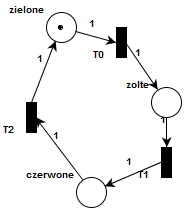
\includegraphics{cw1.png}
\end{center}

Stanami sa miejsca sieci, zaś znacznik pokazuje w jakim stanie aktualnie sie znajdujemy.

\begin{itemize}
    \item Narysować przyklad w symulatorze.
    \item Sprawdzić własciwości sieci (ograniczoność, bezpieczenstwo i możliwy deadlock) w symulatorze Pipe w menu "State Space Analysis".

    \item Wygenerować graf osiągalności "Reachability/Coverability Graph". Zaobserwować: 
    \begin{itemize}[label=$-$]
        \item Jakie znakowania są osiagalne ?
        \item Ile wynosi maksymalna liczba znaczników w każdym ze znakowań ? Jakie mozemy wyciągnac z tego wnioski n.t. ograniczoności i bezpieczenstwa?
        \item Czy kazde przejście jest przedstawione jako krawedz w grafie ? Jaki z tego wniosek n.t. zywotnosci przejsc ?
        \item Czy wychodzac od dowolnego wezla grafu (znakowania) mozna wykonac dowolne przejscie ? Jaki z tego wniosek n.t. zywotnosci sieci? Czy sa mozliwe zakleszczenia ?
    \end{itemize}
    \item Wykonać analizę niezmiennikow (wybrac w menu "Invariant Analysis").
    \begin{itemize}[label=$-$]
        \item wynik analizy niezmiennikow przejsc (T-invariants) pokazuje nam, ile razy trzeba odpalic dane przejscie (T), aby przeksztalcic znakowanie poczatkowege z powrotem do niego samego (wynik nie mowi nic o kolejnosci odpalen). Z wyniku mozemy m.in. wnioskowac o odwracalnosci sieci.
        \item wynik analizy niezmiennikow miejsc (P-invariants) pokazuje nam zbiory miejsc, w ktorych laczna suma znacznikow sie nie zmienia. Pozwala to wnioskowac n.t. zachowawczosci sieci (czyli wlasnosci, gdzie suma znacznikow pozostaje stala) oraz o ograniczonosci miejsc.
    \end{itemize}
\end{itemize}

\section{Rozwiązanie}

\begin{center}
\centering
    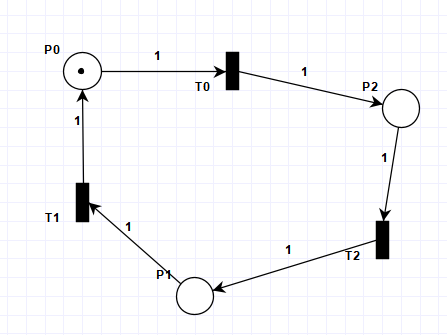
\includegraphics{cw2.png}
    \captionof{figure}{Zbudowany graf w programie PIPE2}
\end{center}

\begin{center}
\centering
    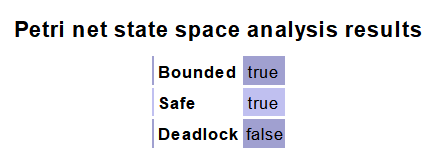
\includegraphics{cw3.png}
    \captionof{figure}{Wyniki "State Space Analysis"}
\end{center}
Jak widzimy sieć jest ograniczona (ponieważ liczba tokenów wewnątrz sieci zawsze jest równa jeden), bezpieczna (jest 1-ograniczona) i nie wystąpi w niej deadlock (nie ma sytuacji, w której nie moglibyśmy przejść dalej).

\begin{center}
\centering
    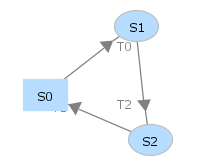
\includegraphics{cw4.png}
    \captionof{figure}{Wyniki "Reachability/Coverability Graph"}
\end{center}
Widzimy, że każde znakowanie jest osiągalne, a maksymalna liczba znaczników w kazdym z nich wynosi jeden. Stąd wniosek, że sieć jest bezpieczna i ograniczona. Każde z przejść jest pokazane jako krawędź w grafie, czyli zawsze można wystartować z dowolnego stanu - oznacza to, że każde przejście jest żywe. Wychodzac od dowolnego znakowania można wykonać dowolne przejście - wynika z tego, że sieć jest żywa oraz nie są możliwe zakleszczenia.

\begin{center}
\centering
    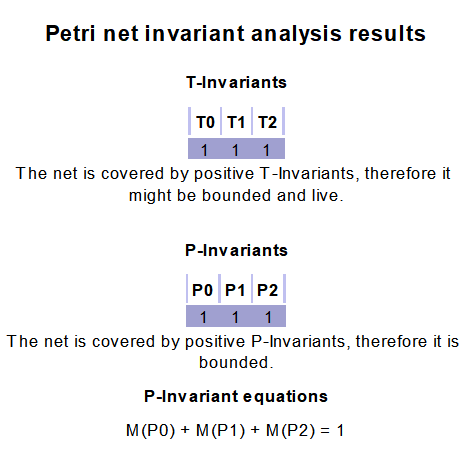
\includegraphics{cw5.png}
    \captionof{figure}{Wyniki "Invariant Analysis"}
\end{center}
Wynik analizy niezmienników przejść mówi, że sieć jest odwracalna, ponieważ, aby wrócić do stanu startowego, należy przejsć przez każdą tranzycję. Z kolei wynik analizy niezmienników miejsc określa miejsca, w których suma znaczników pozostaje stała - sieć jest ograniczona i zachowawcza.

\section{Zadanie 1}
Wymyslic wlasna maszyne stanow, zasymulowac przyklad i dokonac analizy grafu osiagalnosci oraz niezmiennikow j.w.

\newpage
\section{Rozwiązanie}
\begin{center}
\centering
    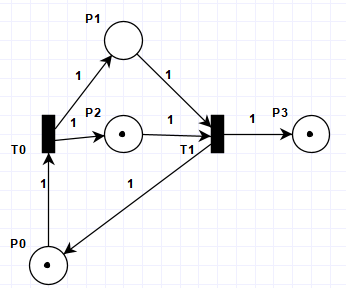
\includegraphics{zad1_init.png}
    \captionof{figure}{Stworzona sieć}
\end{center}

\begin{center}
\centering
    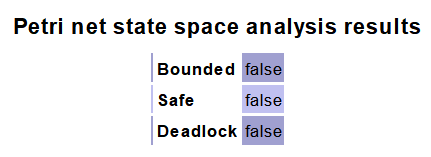
\includegraphics{zad1_state.png}
    \captionof{figure}{Wyniki "State Space Analysis"}
\end{center}
Sieć nie jest ograniczona, ponieważ tranzycja T1 będzie powodować produkowanie dodatkowych tokenów, czyli w miejscu P3, będzie ciągle przybywać tokenów (w nieskończoność). Sieć nie jest bezpieczna ponieważ nie jest 1-ograniczona (w P3 pojawia się więcej niż jeden token). Nie ma możliwości deadlocka, ponieważ zawsze mamy możliwość przejść do innego stanu (poza przechodzeniem z P3).

\begin{center}
\centering
    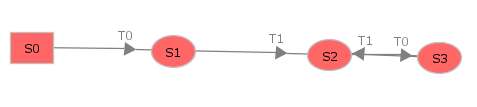
\includegraphics{zad1_reach.png}
    \captionof{figure}{Wyniki "Reachability/Coverability Graph"}
\end{center}
Każde ze znakowań jest osiągalne, każde przejście jest żywe, a więc sieć też jest żywa. 


\begin{center}
\centering
    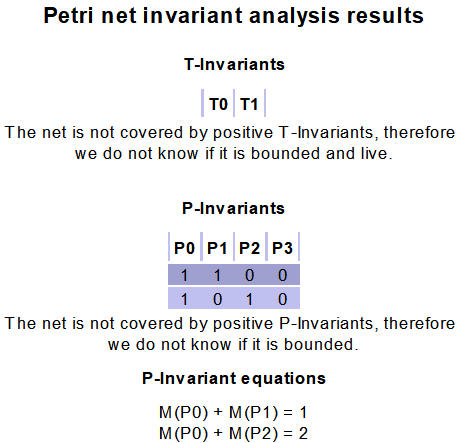
\includegraphics{zad1_invariant.png}
    \captionof{figure}{Wyniki "Invariant Analysis"}
\end{center}
Widzimy, że T-invariants jest puste - stąd wynika, że sieć jest nieodwracalna. Z kolei z równań P-invariants możemy wyciągnąć wniosek, że sieć nie jest bezpieczna, zachowawcza, ograniczona.


\section{Zadanie 2}
Zasymulowac sieć jak ponizej:
\begin{center}
\centering
    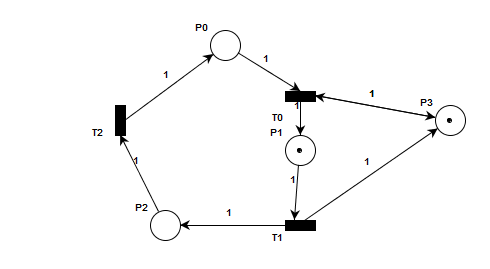
\includegraphics[scale=0.8]{zad2.png}
\end{center}
Dokonac analizy niezmiennikow przejsc. Jaki wniosek mozna wyciagnac o odwracalnosci sieci? Wygenerowac graf osiagalnosci. Prosze wywnioskowac z grafu, czy siec jest zywa. Prosze wywnioskowac czy jest ograniczona. Objasnic wniosek.

\section{Rozwiązanie}
\begin{center}
\centering
    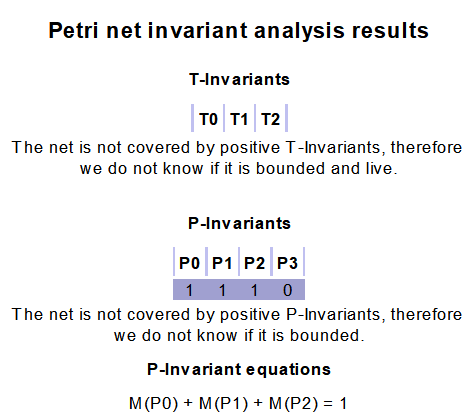
\includegraphics{zad2_invariant.png}
    \captionof{figure}{Wyniki "Invariant Analysis"}
\end{center}

\begin{center}
\centering
    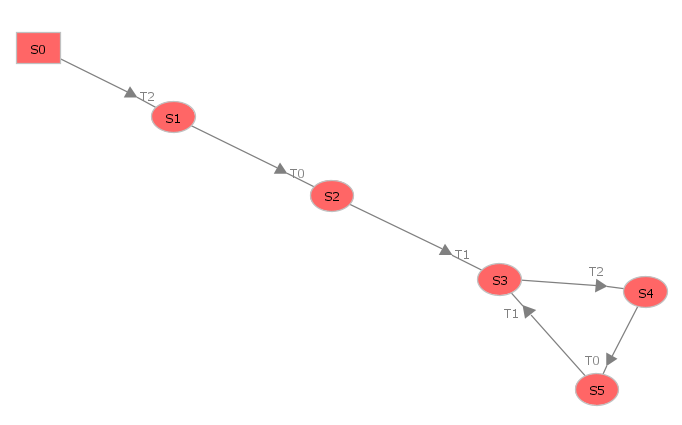
\includegraphics{zad2_reach.png}
    \captionof{figure}{Wyniki "Reachability/Coverability Graph"}
\end{center}

\begin{itemize}
    \item Odwracalność - nie, można to stwierdzić na podstawie wektora (a właściwie jego braku) T-invariants
    \item Żywotność - tak, każde z przejść musi się wykonać, a później wykonują się w pętli
    \item Ograniczoność - nie, ilość tokenów w P3 rośnie w nieskończoność.
\end{itemize}

\section{Zadanie 3}
Zasymulowac wzajemne wykluczanie dwoch procesow na wspolnym zasobie. Dokonac analizy niezmiennikow. Wyjasnij znaczenie rownan (P-invariant equations). Ktore rownanie pokazuje dzialanie ochrony sekcji krytycznej?

\section{Rozwiązanie}
\begin{center}
\centering
    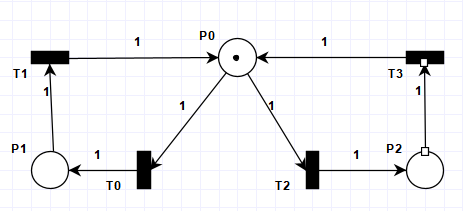
\includegraphics{zad3_init.png}
    \captionof{figure}{Przygotowana sieć przedstawiająca procesy, które wzajemnie się wykluczają}
\end{center}

\begin{center}
\centering
    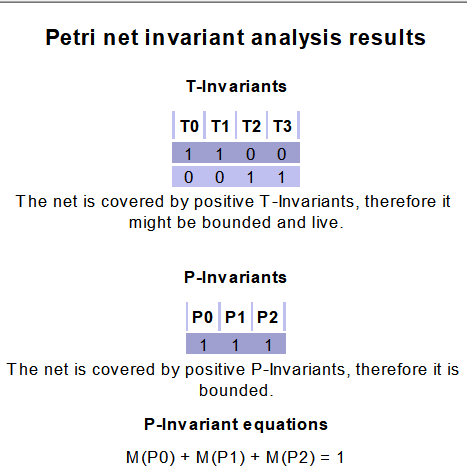
\includegraphics{zad3_invariant.png}
    \captionof{figure}{Wyniki "Invariant Analysis"}
\end{center}

Gdy przyjrzymy się równaniom P-invariant, możemy zauważyć, że występują w nim wszystkie trzy stany. Stan P0 odpowiada za to, że zasób jest wolny, a stany P1 i P2 oznaczają, że zasób jest zajęty przez jeden z procesów. Po prawej stronie równania znajduje się liczba jeden, co oznacza, że suma tokenów we wszystkich stanach zawsze wynosi jeden, czyli token zawsze znajduje się w jednym ze stanów, a na tym polega ochrona sekcji krytycznej.

\section{Zadanie 4}
Uruchomic problem producenta i konsumenta z ograniczonem buforem (mozna posluzyc sie przykladem, menu:file, examples). Dokonac analizy niezmiennikow. Czy siec jest zachowawcza? Ktore rownanie mowi nam o rozmiarze bufora?

\section{Rozwiązanie}
\begin{center}
\centering
    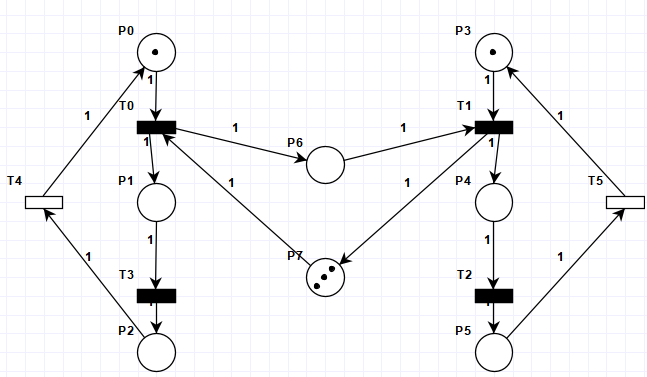
\includegraphics{zad4.png}
    \captionof{figure}{Problem producenta i konsumenta z ograniczonym buforem}
\end{center}
\begin{center}
\centering
    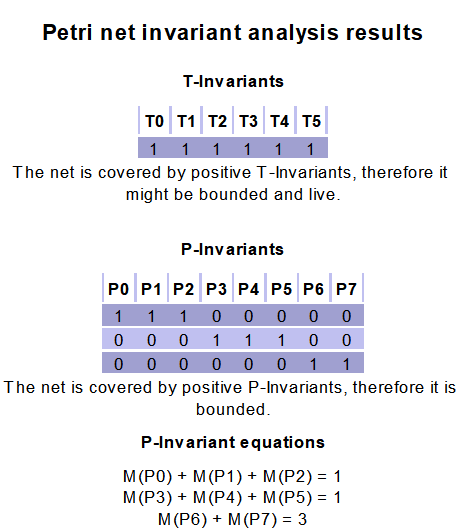
\includegraphics{zad4_invariant.png}
    \captionof{figure}{Wyniki "Invariant Analysis"}
\end{center}

Sieć jest zachowawcza, ponieważ każda tranzycja produkuje tyle samo tokenów ile pobiera. Na podstawie wektora T-invariants widzimy, że sieć jest odwracalna. Sieć jest żywa gdyż wszystkie przejścia mogą być wykonane. O wielkości bufora mówi nam równanie nr. 3. Stan P6 odpowiada za miejsca zajęte, a P7 za miejsca wolne.

\section{Zadanie 5}
Stworzyc symulacje problemu producenta i konsumenta z nieograniczonym buforem. Dokonac analizy niezmiennikow. Zaobserwowac brak pelnego pokrycia miejsc.

\section{Rozwiązanie}
\begin{center}
\centering
    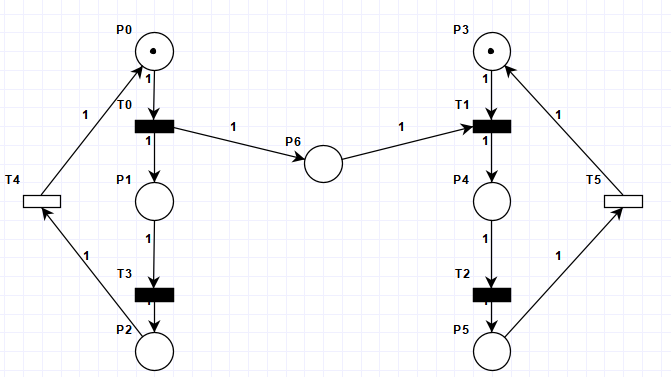
\includegraphics{zad5_init.png}
    \captionof{figure}{Problem producenta i konsumenta z nieograniczonym buforem}
\end{center}
\begin{center}
\centering
    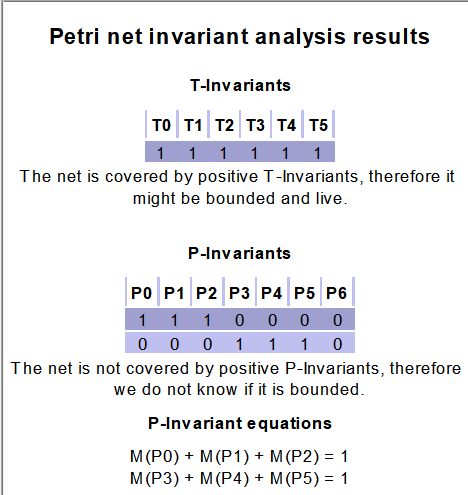
\includegraphics{zad5_invariant.png}
    \captionof{figure}{Wyniki "Invariant Analysis"}
\end{center}
Z wektora T-invartiants - sieć odwracalna. Jest też żywa, ponieważ każdy stan jest osiągalny. W sekcji P-invariant equations obserwujemy, brak wystąpienia stanu P6, czyli bufora. Jest tak dlatego, iż jest on nieograniczony i nie da się go określić równaniem. Pozostałe równania opisują procesy wytwarzania i konsumowania tokenów.

\section{Zadanie 6}
Zasymulowac prosty przyklad ilustrujacy zakleszczenie. Wygenerowac graf osiagalnosci i zaobserwowac znakowania, z ktoroch nie mozna wykonac przejsc. Zaobserwowac wlasciwosci sieci w "State Space Analysis". Ponizej przyklad sieci z mozliwoscia zakleszczenia (mozna wymyslic inny):

\section{Rozwiązanie}
\begin{center}
\centering
    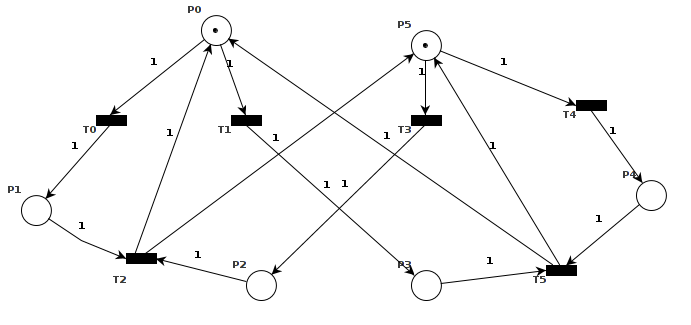
\includegraphics{zad6_init.png}
    \captionof{figure}{Zamodelowana sieć}
\end{center}
\begin{center}
\centering
    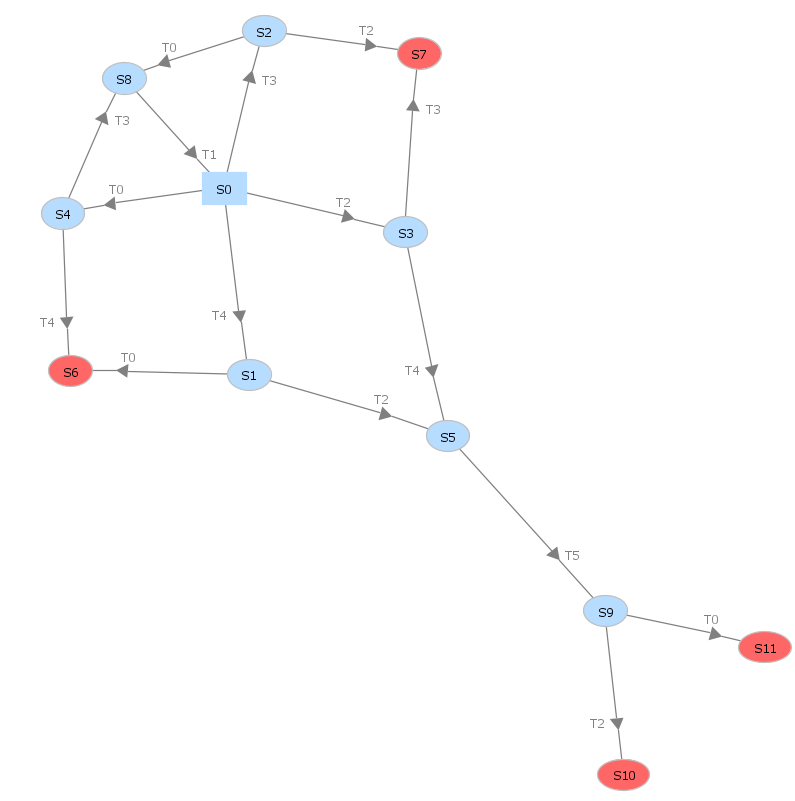
\includegraphics{zad6_reach.png}
    \captionof{figure}{Wyniki "Reachability/Coverability Graph"}
\end{center}
Graf pozwala jednoznacznie stwierdzić, że stanami, w których nastąpi deadlock są stany: S6, S7, S10, S11 - wchodząc do nich nie można już przejść dalej. Wynik analizy "State Space" pozwala poznać najkrótszą ścieżkę prowadzącą do zakleszczenia.

\begin{center}
\centering
    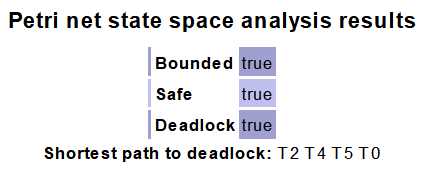
\includegraphics{zad6_state.png}
    \captionof{figure}{Wyniki "State Space Analysis"}
\end{center}

\section{Wnioski}
Powyższe przykłady ukazują, że sieci Petriego pozwalają modelować różne systemy. Procesy zazwyczaj przebiegają według jakiegoś określonego modelu, dzieki temu możemy zbadać właściwości tego procesu, a dzięki temu poznać zależności między poszczególnymi podsystemami. Sieci Petriego pozwalają także unaocznić przebieg i zakończenie danego systemu, co może być użyteczne w wyszukiwaniu problemów (np. zakleszczeń). 

\section{Bibliografia}
\begin{itemize}
    \item \url{http://jedrzej.ulasiewicz.staff.iiar.pwr.wroc.pl/ProgramowanieWspolbiezne/wyklad/Sieci-Petriego15.pdf?fbclid=IwAR3euBljzKlFJS0nbfJpHYjRgv8tzs_rAG7fSj84x2too3zE7nf5JaOb2yA}
    \item \url{http://sirius.cs.put.poznan.pl/~inf89721/MiAPB/Nowe/5%20-%20Analiza%20sieci%20Petriego.pdf}
    \item \url{https://pl.wikipedia.org/wiki/Sie%C4%87_Petriego#:~:text=Sie%C4%87%20Petriego%20%E2%80%93%20j%C4%99zyk%20modelowania%20dyskretnych,zosta%C5%82y%20zdefiniowane%20w%20latach%2060.}
    \item \url{http://robert.wojcik.staff.iiar.pwr.wroc.pl/dydaktyka/dzienne/ina/miasi_l1.pdf}
\end{itemize}

\end{document}
